%%% SOME OF THIS CODE IS ADAPTED FROM THE VENERABLE withesis.cls

%% BEGIN PAGESTYLE

%%% You can pick a pagestyle if you want; see the memoir class
%%% documentation for more info.  The default ``deposit'' option meets
%%% the UW thesis typesetting requirements but is probably
%%% unsatisfactory for making a version of your dissertation that
%%% won't be deposited to the graduate school (e.g. for web or a nice
%%% printed copy)

\chapterstyle{deposit}
\pagestyle{deposit}

\chapter{Research Overview}

%The goal of my research is to enable animators to easily author directed gaze animation for virtual characters that looks plausible and communicates effectively. I propose a robust, cost-effective approach that is based on the idea of representing the gaze behavior as a sequence of gaze shifts and providing techniques for automated synthesis and easy manual editing of this sequence. The components of the work are: (1) a procedural, parametric model for synthesis of individual gaze shifts; (2) stylized gaze techniques for adapting gaze shift motion to a range of character designs; (3) authoring approach for obtaining plausible directed gaze for an input body motion and environment; (4) an extension to this approach for authoring effective directed gaze that satisfies animator-specified communicative goals; (5) a study with human participants evaluating the effectiveness of authored gaze behaviors in the context of task demonstrations with a virtual agent. I give an overview of each component in the following sections.

\section{Animating Directed Gaze Shifts (completed)}
\label{sec:GazeShifts}

I define a directed \emph{gaze shift} as a coordinated movement of the character's eyes, head, and torso toward a target in the environment, which is followed by a \emph{gaze fixation} of the target. In my approach, gaze shifts serve as building blocks of larger gaze patterns that achieve specific communicative effects. The first step of my research was then to enable animation of individual gaze shifts. To that end, we have developed a procedural, parametric model for gaze shift synthesis. Originally developed as an eye-head coordination model by~\citet{andrist2012headeye}, we have further extended it with support for coordinated upper body movement. The model is implemented as a procedural, dynamic, feed-forward animation controller that synthesizes rotational motion of the eyes, head, and torso joints toward the target using a set of kinematic laws derived from studies of primate gaze in neurophysiology~\citep{guitton1987gaze,mccluskey2007monkeys}. The use of neurophysiology-based kinematics enables the model to synthesize gaze motion that looks \emph{plausible}, while retaining the key advantage of procedural models---high degree of control.

The gaze shift model accepts as input the properties of the gaze shift that should be synthesized, which include gaze target location (3D point in space where the agent will look) and head and torso
\emph{alignment parameters}. The latter parameters specify how far each of these body parts will rotate relative to the target. For example, low head alignment specifies that the character should only minimally turn its head toward the target and look at it ``out of the corner of the eye'', whereas high head alignment means the character will face the target straight on (Figure~\ref{fig:HeadTorsoAlignment}). The idea of alignment parameters is to enable the animator to control the character's attention signal: by turning its head and torso more toward a target, the character communicates a higher level of attention toward the target. The ability to parametrically control how the gaze shift communicates attention is a key to creating \emph{effective} directed gaze. The intuitive gaze parametrization also makes the model \emph{cost-effective} with respect to animator effort and skill, because the animator does not need to worry about the timing of eye, head, and torso movements.

\begin{figure*}
\centering
\includegraphics[width=1\textwidth]{figures/HeadTorsoAlignment.pdf}
\caption{Examples of gaze shifts synthesized using our model: (1) The agent maintaining eye contact with the viewer. (2) Gaze shift to the side with low value of the head alignment parameter. (3) Gaze shift in the same direction, but with high head alignment value. (4) Gaze shift in the same direction with a small shift in torso posture. (5) As before, but with a large shift in torso posture.}
\label{fig:HeadTorsoAlignment}
\end{figure*}

\subsection{Evaluation}

The original head coordination model was evaluated in prior work~\citep{andrist2012headeye,andrist2012designing}, demonstrating its \emph{plausibility} (measured as perceived naturalness of observed gaze shifts~\citep{andrist2012headeye}) and communicative \emph{effectiveness} (measured respectively as accuracy of participants' guesses at the character's attention direction~\citep{andrist2012headeye} and the effects of head alignment on information recall, engagement, and subjective perceptions of the character~\citep{andrist2012designing}.)

Following our extensions of the model to torso movements, we conducted another evaluation measuring the effects of torso alignment. In the study, we had a virtual character perform a series of gaze shifts toward gaze targets (paintings) in its virtual environment with varying levels of torso alignment (Figure~\ref{fig:TorsoAlignStudyConditions}). For each set of paintings, the participants were asked to rate how interested the character appeared to be in each painting---perceived interest serving as a measure of the strength of torso orientation as an attention cue. Results showed that the more the character aligned its torso with a particular painting, the more interested she was perceived to be in that painting, thereby demonstrating the model's \emph{effectiveness}.

\begin{figure*}
\centering
\includegraphics[width=0.85\textwidth]{figures/TorsoAlignStudyConditions.pdf}
\caption{Conditions in the evaluation of our gaze shift model.}
\label{fig:TorsoAlignStudyConditions}
\end{figure*}

\section{Stylized Gaze (completed)}
\label{sec:StylizedGaze}

Gaze shift models such as the one developed in my own work (Section~\ref{sec:GazeShifts}) produce plausible gaze motion because they are based on the kinematics of real human gaze. As such, they implicitly incorporate biomechanical and neurophysiological constraints of the human visuomotor system. Applying these models to characters with non-humanlike designs, such as stylized characters found in animated films, would result in gaze motion that contains anomalous and distracting visual artifacts---in other words, it would no longer look \emph{plausible}. However, the ability to animate the gaze of stylized characters is important: stylization affords a way to emphasize and exaggerate the character's personality traits, enhance their appeal, and avoid uncanny valley effects that can occur in realistically designed characters~\citep{geller2008overcoming}. A \emph{robust} animation approach should be able to handle such varied character designs.

As part of this research thread, we identified visual artifacts that occur when animating characters with stylized designs with neurophysiologically accurate movements synthesized by our gaze shift model (Section~\ref{sec:GazeShifts}) and we developed techniques for adapting the movements such that artifacts are avoided. We refer to these techniques as \emph{stylized gaze}~\citep{pejsa2013stylized}. For example:

\begin{itemize}
\item Characters with large eyes set wide apart appear cross-eyed when focusing on a nearby target (Figure~\ref{fig:CrossEyedness}, left); we deal with this artifact by moving the effective location of the target further away from the character and thereby reducing the convergence angle of the eyes (Figure~\ref{fig:CrossEyedness}, right).
\item Characters with asymmetric eyes suffer from disconjugate eye movements. Asymmetric eyes have different motor range (OMR) in different directions. If both eyes move at the same velocity (as is the norm for human gaze), then one of the eyes reaches its OMR limit sooner and becomes ``stuck'', while the other eye continues to move (Figure~\ref{fig:StuckEye}), which appears anomalous. Our solution is to adjust eye kinematic such that the eye that has a shorter distance to cover moves more slowly and both eyes reach OMR at the same time.
\end{itemize}

\begin{figure*}
\centering
\includegraphics[width=0.75\textwidth]{figures/CrossEyedness.pdf}
\caption{Left: A stylized character with large eyes appears cross-eyed when focusing on a nearby target. Right: Our adaptation techniques remove the artifact by reducing the eyes' convergence angle.}
\label{fig:CrossEyedness}
\end{figure*}

\begin{figure*}
\centering
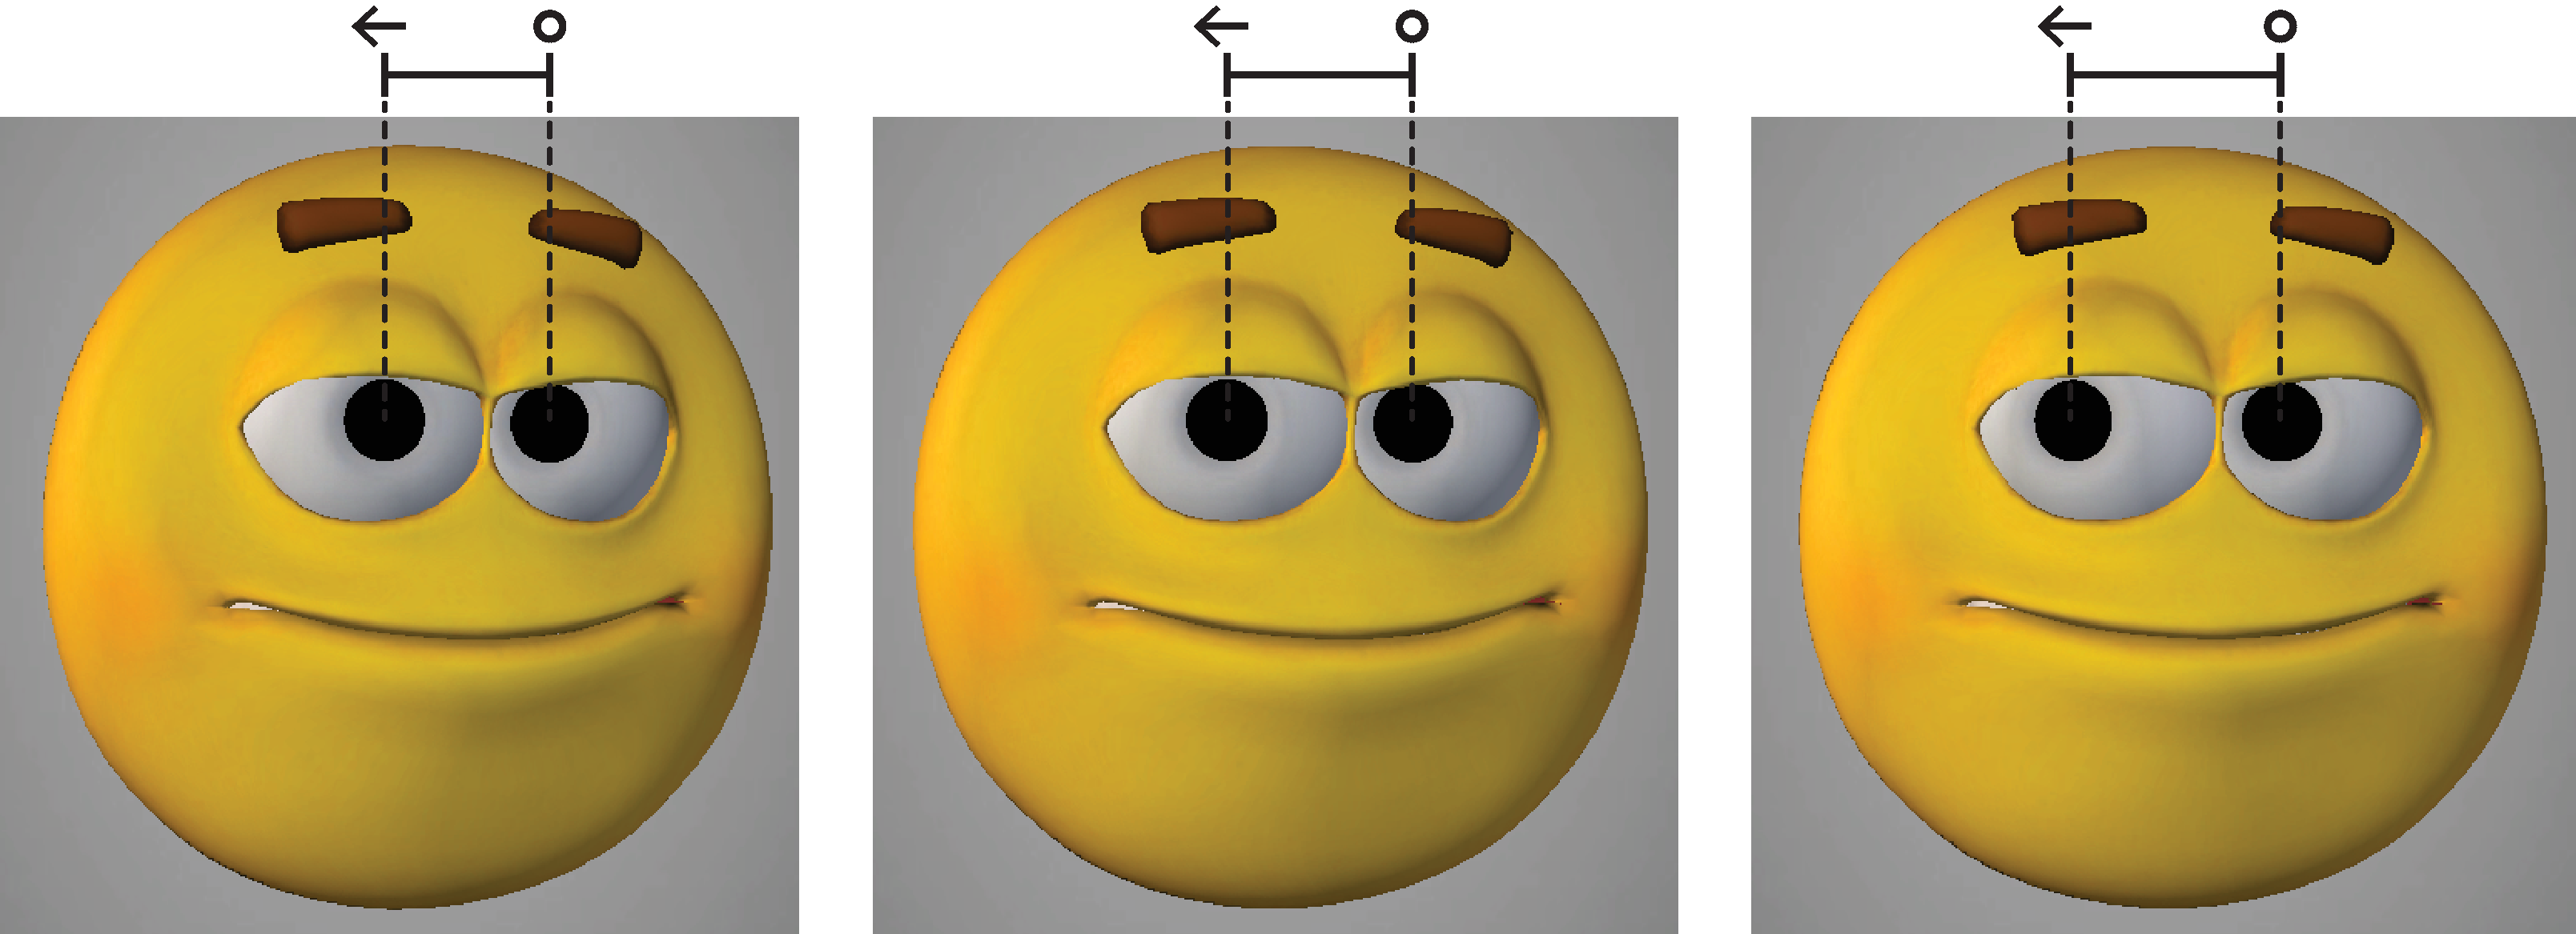
\includegraphics[width=0.75\textwidth]{figures/StuckEye.pdf}
\caption{Disconjugate eye movements due to asymmetric eye shape. The right eye is moving ahead,
while the left eye is blocked at OMR limit. Notation: Dot $\circ$ indicates that the left eye is stationary.}
\label{fig:StuckEye}
\end{figure*}

\subsection{Evaluation}

Stylized gaze techniques produce poses and movements that look \emph{plausible} by removing animation artifacts, and they do so in a \emph{robust} way, which means they should perform well on morphologically varied characters. To verify these claims, we performed a simulation where we synthesized a variety of gaze shifts across a range of characters and we quantitatively measured the prevalence of animation artifacts in these examples, finding that artifact prevalence is greatly reduced when using stylized gaze techniques.

Moreover, stylized gaze techniques depart from biomechanically valid human gaze, so we needed to verify whether this departure has any impact on the communicative function of gaze---i.e., whether attention direction is still accurately communicated following adaptation to a stylized character. We conducted a study where participants were shown videos of characters with realistic and stylized morphologies performing gaze shifts toward targets in the environment and asked to infer what target the character was gazing at. We found that adapted gaze shifts had the same accuracy as unadapted gaze on a realistically proportioned character, demonstrating that they remained \emph{effective}.
%In the same study, we asked the participants to rate the naturalness of gaze shifts in various conditions (using the same naturalness measure employed in~\citet{andrist2012headeye}) and  found no significant effect. This result suggests that gaze shift motion adapted by our techniques has the same \emph{plausibility} as unadapted gaze on a realistic character, but it also suggests that animation artifacts of unadapted gaze on a stylized character had no impact on plausibility that we could detect by the chosen measure.

\section{Authoring Plausible Directed Gaze (ongoing)}
\label{sec:GazeAuthoring}

The focus of my work is on animating gaze in scenarios involving a character performing some actions in a virtual environment---Figure~\ref{fig:PlausibleGazeAuthoring} shows two examples. With growing availability of low-cost, low-volume motion capture, such scenarios are becoming increasingly cost-effective to produce. However, this cost-effectiveness only extends to capturing body motion, while authoring gaze animation remains a challenge. Typical motion capture setup does not record eye movements (separate eye tracking technology is required for that purpose) and editing the character's gaze is frequently necessary to correct for errors in the performance and modify its content. My proposed solution is a gaze authoring approach that, given an input body motion and environment, automatically infers a directed gaze behavior that looks \emph{plausible}.

The basis of our authoring approach is a concise representation of directed gaze as a temporal sequence of \emph{gaze annotations} accompanying the original motion, where each annotation describes a gaze shift toward a target in the environment, followed by fixation of that target. Annotations specify only the basic timing and posture properties of the gaze shift while abstracting away motion details. Actual gaze shift kinematics are synthesized automatically by a gaze controller using our neurophysiology-based gaze shift model (Section~\ref{sec:GazeShifts}), which ensures that the resulting animation looks plausible given the specification. The representation based on gaze annotations forms the backbone of our gaze authoring system: we provide (1) methods for automated \emph{inference} of annotations from motion capture data, (2) an accessible graphical tool for manual \emph{editing} of the annotations, and (3) a robust approach for \emph{synthesis} of natural gaze movements from the annotation sequence:

\begin{enumerate}
\item \emph{Gaze inference} model infers a plausible directed gaze behavior for the given body motion and environment by analyzing the properties of the body motion signal. The model searches the motion signals of the head and torso joints for occurrences of the characteristic gaze shift kinematic profile (reported in~\citep{pejsa2015gaze}) to infer gaze shift timings, and it analyzes the facing direction of the head to infer the location of the likely gaze target in the environment. This inferred information is encoded in gaze annotations, from which the corresponding gaze animation is synthesized (item 3). Figure~\ref{fig:PlausibleGazeAuthoring}, left illustrates an example of adding inferred gaze to a captured body motion.
\item \emph{Gaze editing} tool enables modification of the gaze behavior by editing the annotations. Animator can use a graphical tool, implemented as an add-on for Unity game engine (Figure~\ref{fig:GazeEditingTool}), to add or remove gaze shifts toward specified targets, adjust gaze shift timings, fine-tune head and torso postures via alignment parameters, and edit gaze indirectly by editing the environment and gaze target layout. Figure~\ref{fig:PlausibleGazeAuthoring}, right shows an example of characters' gaze behaviors edited by adding gaze toward a new target.
\item \emph{Gaze synthesis} techniques generate gaze shift movements from the annotation sequence and layer them onto the character’s body motion. For each annotation, our gaze controller synthesizes a coordinated eye, head, and torso movement toward the specified gaze target. The synthesized movement is layered onto the body motion such that elements of the original body posture are preserved, and an inverse kinematics solver is employed to preserve end-effector constraints, which can become violated due to changes in torso posture effected by gaze. The result is a final character motion that incorporates the gaze behavior while preserving expressive properties and kinematic constraints of the original motion.
\end{enumerate}

\begin{figure*}
\centering
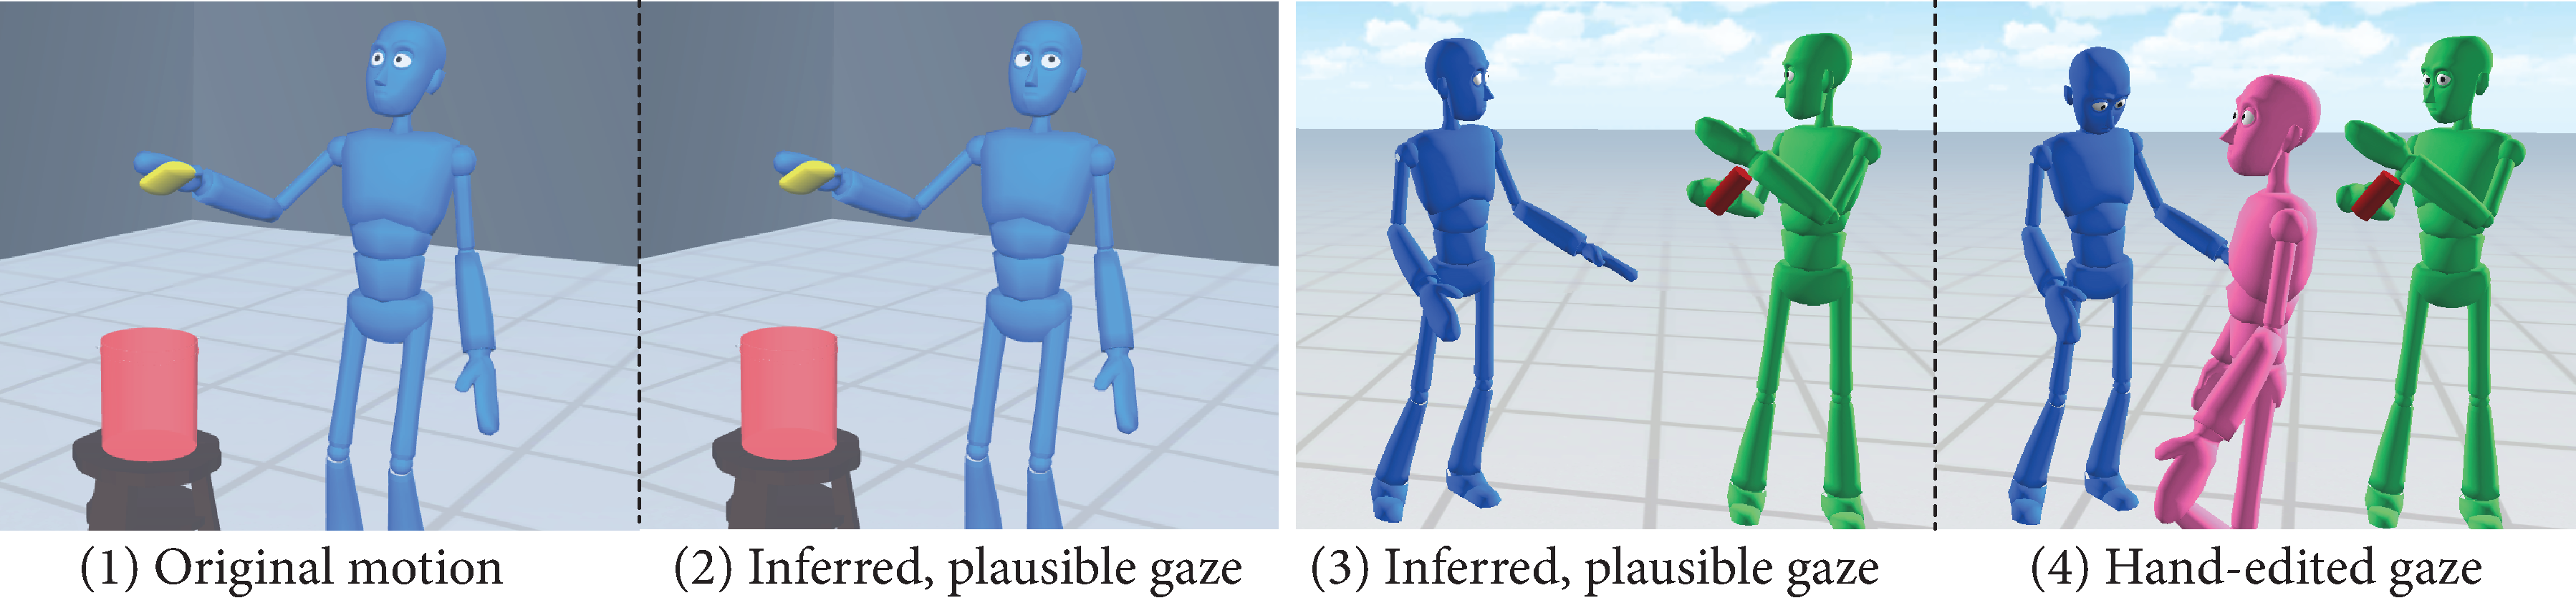
\includegraphics[width=1\textwidth]{figures/PlausibleGazeAuthoring.pdf}
\caption{Examples of directed gaze created using our approach for plausible gaze authoring. From left to right: (1) Original, captured body motion. (2) Our system has automatically inferred and added plausible gaze to the original motion. (3) Motion with plausible, unedited gaze. (4) Added gaze toward a new character using our editing tool.}
\label{fig:PlausibleGazeAuthoring}
\end{figure*}

\begin{figure*}
\centering
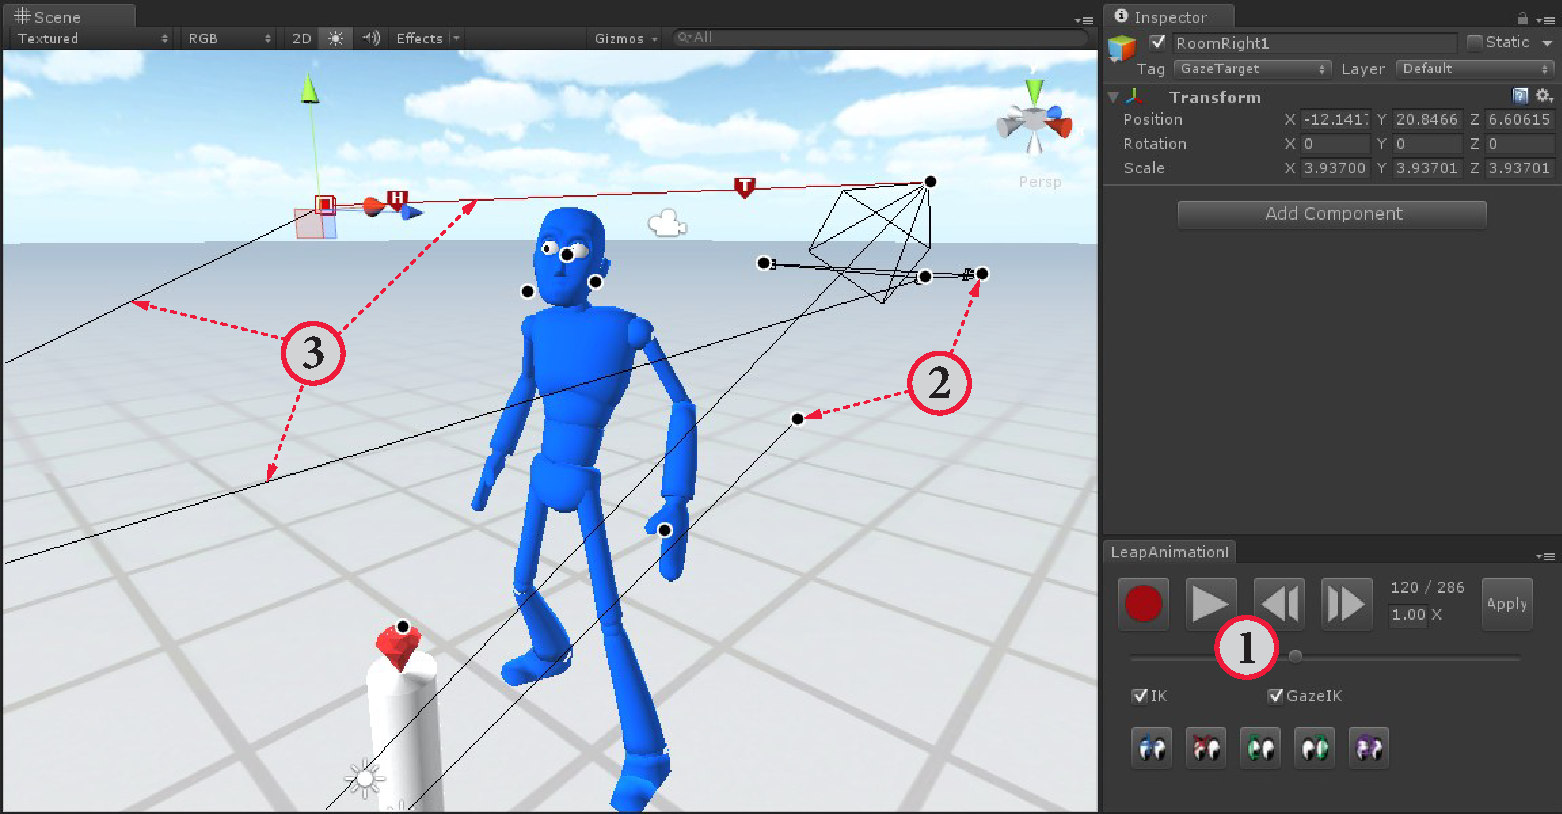
\includegraphics[width=1\textwidth]{figures/GazeEditingTool.pdf}
\caption{Graphical tool for hand-editing directed gaze. (1) Controls for animation playback and editing operations. (2) Dots indicate gaze targets in the virtual environment. (3) Directed lines connecting the targets represent gaze shifts.}
\label{fig:GazeEditingTool}
\end{figure*}

The directed gaze model supported in our approach is not a comprehensive model of human gaze. Real human gaze involves other types of movements, such as smooth pursuit, random saccades, and eye blinks. Smooth pursuit movements occur in specific situations, such as visual tracking of moving objects---while we presently have no plans to incorporate them, they have been computationally modeled in prior work~\citep{yeo2012eyecatch} and could be integrated in our system. However, eye blinks and random saccades occur constantly, so we have modeled them in our system (we use the Eyes Alive model for saccades~\citep{lee2002eyes}) and we generate them probabilistically as part of the synthesized gaze behavior. Eye blinks and saccades introduce non-deterministic variety into the otherwise deterministic directed gaze behavior and thus contribute to its plausibility.

\subsection{Evaluation}

We have demonstrated the gaze authoring approach on a range of scenarios, including multi-character interactions, walking around an environment, and complex environment interactions. To evaluate the \emph{cost-effectiveness} of the approach, we had an experienced animator author gaze animation in several scenarios using a traditional keyframing workflow and we measured the required effort as the number of required operations (set keyframes), which we compared to the number of operations used in our own tool. In one example, the animator had to set 143 keyframes to animate just the eyes, while our system could synthesize a similar estimate of eye movements completely automatically.

It still remains to conduct an evaluation of \emph{robustness} and \emph{plausibility} of the resulting gaze animation. One possible approach is to measure plausibility as overlap between inferred gaze behavior and some ground truth for a range of motions. Motions with hand-animated gaze could be used as ground truth or new motions could be captured while using an eye tracker to obtain their actual eye movements. Another approach is to measure plausibility in a study as participants' aesthetic preference for motions with inferred gaze. On each trial of the task, the participant would be shown two versions of the motion from a pool of three (original motion without gaze, motion with inferred gaze, motion with ground-truth gaze) and asked to choose which one they like better. Significant preference for inferred gaze over no gaze would be sufficient evidence of plausibility, further strengthened if there were no significant preference for ground-truth gaze over inferred gaze. Both studies need to be conducted with a large and varied pool of motions to also verify the \emph{robustness} of the approach.

\section{Authoring Effective Directed Gaze (planned)}
\label{sec:GazeBehaviorSynthesis}

The gaze authoring approach proposed in Section~\ref{sec:GazeAuthoring} can automatically produce gaze behavior that looks \emph{plausible}, but not \emph{effective}, because the inference model has no notion of communicative effects that the gaze behavior should trigger. To support such effects, the animator would need to use the manual editing tool to introduce specific gaze patterns into the original behavior. For example, to make the character's gaze more engaging, the animator would need to manually add gaze shifts toward the camera throughout the scenario. That is not the most \emph{cost-effective} approach, as the number of operations required increases linearly with scenario length, and a degree of expert knowledge is required, since the animator must know which gaze patterns yield the desired effects in communication. Ideally, it should be possible to have the animator specify the desired communicative effects once and then automatically synthesize the gaze patterns that achieve them. In this section, I discuss an extension to the gaze authoring approach that meets this objective.

%I will further augment the proposed authoring approach with a new automated synthesis model producing gaze behavior that is not only plausible for the current animated scenario, but also \emph{effective} given the animator-specified communicative goals. The model will expose a set of attention parameters enabling the animator to easily specify how the character should distribute its attention among the viewer and task objects, allowing automated synthesis of gaze patterns that optimize for effects such as improved engagement or understanding of task information.
I propose a new gaze inference model that accepts low-level inputs (body motion and environment, as well as a small set of high-level \emph{attention parameters}. The attention parameters will let the animator specify how the character should distribute its attention over the course of the interaction, allowing them to design a gaze behavior with specific effects on the viewer. One subset of parameters will be \emph{gaze posture parameters}, which will influence how the character distributes its head and body posture between the viewer and environment via the gaze shift model's head and torso alignment parameters. Another subset will be \emph{gaze pattern parameters}, which will control the probability of a particular gaze pattern, including: (1) \emph{affiliative gaze}, where the character predominantly looks at the viewer, potentially leading to greater engagement of the viewer and more positive perceptions of the agent; (2) \emph{referential gaze}, where the character alternates between looking at viewer and signaling their referential or action intent toward environment objects, resulting in potentially better recall of information grounded in those objects (Figure~\ref{fig:SandwichMaking}); (3) \emph{neutral gaze}, where the character focuses on the environment and does not gaze at the viewer at all.

\begin{figure*}
\centering
\includegraphics[width=1\textwidth]{figures/SandwichMaking.pdf}
\caption{Example scenario where the actor demonstrates the process of making a sandwich. Actor is displaying a gaze pattern characteristic of \emph{referential gaze}, consisting of gaze toward the viewer (left), followed by a gaze shift toward the next ingredient (middle) that grounds the linguistic reference to the ingredient and signals the intent to pick it up, and ending with a gaze shift back to viewer (right).}
\label{fig:SandwichMaking}
\end{figure*}

The new gaze inference model will compute a gaze behavior (expressed as a sequence of annotations) that is as close as possible fit to the given body motion, environment, and attention parameter values. The model could be implemented as a hill-climbing, state-space search, where states correspond to various gaze shift sequences describing the complete gaze behavior. The initial state for the search could be the output of the original gaze inference (using just the body motion and environment as inputs)---which we know to be a plausible gaze behavior---and neighboring solutions could be generated by probabilistically adding and removing gaze shifts and evaluating their fitness with respect to the body motion, environment, and attention parameter settings.

\subsection{Evaluation}

Evaluation of the complete gaze authoring approach will constitute a separate research contribution; I discuss it in the next section.

\section{Effective Directed Gaze for Virtual Demonstrators (planned)}
\label{sec:DemonstratorsGaze}

In the final project, I will apply the gaze authoring approach to a concrete application---animating directed gaze of virtual agents performing physical task demonstrations, such as assembly, repair, and operation of various devices and machinery. This project will serve as an evaluation of the \emph{effectiveness} of directed gaze synthesized by the approach and \emph{robustness} of the approach with respect to different attention parameter settings, and it will also constitute a larger contribution by informing the design of gaze behaviors for animated agents in an educational setting. Previous research has shown that virtual agents and social robots with appropriately designed gaze patterns can facilitate better information recall in scenarios such as storytelling~\citep{mutlu2006storytelling} and lecturing~\citep{andrist2012designing}. Findings from these studies suggest that increased gaze from the agent can lead to improved information recall and that head alignment during gaze has effects on information recall, engagement, and positive perceptions of the agent.

Designing the agent's gaze behavior in a physical task demonstration is challenging from the standpoint of authoring \emph{robustness} and \emph{cost-effectiveness}. Such a demonstration is likely to involve a lot of interaction with task objects in the environment. Appropriate gaze behavior in such scenarios will involve gaze toward relevant objects as they are discussed or handled by the demonstrator. On the other hand, the demonstrator should also gaze toward the viewer to make the demonstration more immediate and engaging, and to initiate joint attention toward important task objects. An effective virtual demonstration requires a complex interplay of gaze patterns that are difficult to author manually. Furthermore, this complex gaze behavior must be layered onto the complex, contact-rich body motion and adapted to the spatial layout of task objects. Prior studies of gaze tended to focus on storytelling and lecturing scenarios with little environment interaction and therefore simpler body motions and gaze patterns. Our gaze synthesis approach will be able to infer appropriate gaze patterns in an automated and therefore \emph{cost-effective} way, and it will be \emph{robust} to variation and complexity in body motion and environment layout. The application of the approach to the problem of virtual demonstrations will also serve as a demonstration of robustness and cost-effectiveness.

My proposed plan for the current research thread is to conduct a study with human participants to investigate the effects of the virtual demonstrator's gaze behavior on the effectiveness of their demonstration. We will devise model assembly and repair tasks---i.e., tasks designed to be mechanically  similar to real-world assembly and repair---and capture a human performing demonstrations of these tasks. A model assembly task might be constructing a specified shape out of toy blocks, while a model repair task might be correcting a mistake in a previously assembled shape. Next, we capture a demonstrator performing these tasks using a motion capture setup built for this purpose. For example, Figure~\ref{fig:SandwichMaking} illustrates an assembly task being captured with a markerless setup consisting of a pair of Kinect 2 devices and a head-worn eye tracker. Given the captured motion and a 3D model of the task environment, we will use our gaze authoring approach to synthesize the directed gaze animation to match the captured performance and reconstructed task environment. We will manipulate the gaze inference model's attention parameters to yield gaze behaviors designed to maximize viewer engagement (affiliative gaze) and task understanding (referential gaze). These gaze behavior variations will serve as distinct conditions in our study.

We will show the virtual demonstrations as stimuli to our participants and we will measure their effects on participants' (1) task understanding, (2) engagement, (3) perception of the demonstrator's credibility and competence, and (4) attention. To measure \emph{task understanding}, we will employ an objective measure, such as a questionnaire measuring information recall or having the participants perform the task and measuring completion time. For measuring \emph{engagement} and perceived \emph{credibility} and \emph{competence} we can employ previously validated subjective questionnaires from studies such as~\citep{andrist2012designing}. Finally, to truly explain how the agent's gaze patterns shape participants' understanding and subjective experience of the task, we must understand their effect on participants' \emph{attention} over the course of the demonstration---we can measure the latter by monitoring the participant's own gaze patterns using an eye tracker. 